\chapter{The LTLCreator prototype}

As stated in chapter~\ref{chap:goals}, appropriate support by a graphical editor is important for the usefulness of the developed visual language. We therefore designed and implemented a prototype of such an editor. The proposed constraint generation heuristics is integrated in this prototype as well and could thus be evaluated. The implementation is a java swing component, making it easy to integrate the visual language into other java applications. An API enables an underlying state machine which also influences the state propositions available for constraint editing. Furthermore a particular model checker can be specified for constraint validation. As a default, the symbolic model checker NuSMV~\cite{springerlink:10.1007/s100090050046,NuSMV2} is used.

Fig.~\ref{fig:editor} shows a snapshot of the editor's environment: All functionality needed for constraint editing is provided in the tool bar on the right. It contains draggable elements for creating all operator and proposition types as well as a trashcan for deleting. Constraints can be composed in the dashboard in the center of the editor by drag\&drop. The tab functionality on the left allows multiple constraints to be managed. Each tab shows a small thumbnail of the constraint and a symbol indicating its validity (a warning shield for ``incomplete'', a green shield for ``valid'', a red cross for ``invalid'' or an animated ring for ``validation in progress.'') The magic wand button within the tab pane triggers the constraint generation.

\begin{figure}[htbp]
  \centering
  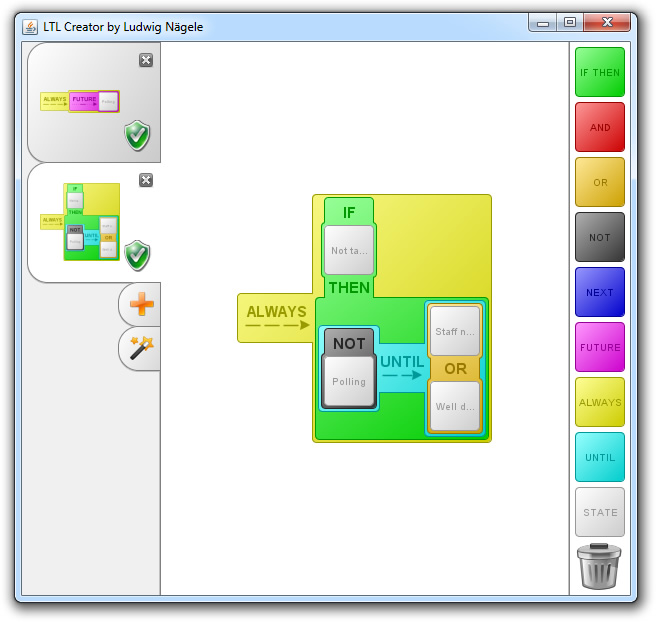
\includegraphics[width=\linewidth]{editor} 
  \caption{Snapshot of the visual editor.}
  \label{fig:editor}
\end{figure}

TODO: Kleine Inhaltsangabe



\section{Operator constraints}
\section{Automated constraint generation}


% (on huge state machines) (brute force algorithm)
 
%Da der subgraph-finde-algorithmus als brute force algorithmus implementiert wurde, der saemtliche sub graphs durch Abwandern s�mtlicher Pfade der zugrundeliegenden state machine herauszufinden versucht, kann bei grossen programmen (ab ca. 1000 Zustaenden und sehr vielen Verzweigungen) der findeprozess teils sehr lange (mehrere Minuten) dauern. Um den warteprozess ertraelicher zu machen wird w�hrend der findung ein dialog mit dem aktuellen fortschritt und einem abbrechen button angezeigt.

\section{Model checker}

NuSMV
warum den? Davor verwendete erwaehnen?






\section{Interaction with Robostudio}

allein benutzbar, oder ueber robostudio, automatische synchronisierung mit model

%Since Robostudio uses NetBeans as a platform, the LTLCreator has to be integrated as a NetBeans component. Die Datenanbindung zum Austausch des modells (Zustandsmaschine) und der Constraints erfolgt hierbei durch �ffentliche




\subsection{Problems}

(auto-revalidation, model-errors, ...?)
nicht EINE zentrale stelle f�r model�nderungen => zer\-pfl�ck\-te programmierung, wenn man alle �nderungen haben will




\subsection{Solutions}

(pre-checker)

statische analyse